\chapter{灵长类动物前额叶皮层的进化}

\section{概述}
前额皮层的进化经历了不同的阶段。早期哺乳动物经历了一次进化,产生了所有哺乳动物共有的颗粒状前额(后文简称PF)区域。这些区域的产生能根据预测结果改善行动(第3章)和对象(第4章)之间的觅食选择。
早期灵长类动物经历了另一个进化,形成了第一个颗粒状的PF区域。
原本这些动物的仅在夜间生活于细小的树枝上,它们在那里寻找、选择和获取食物,用一种需要头部和一只手协调运作的方法进食。
他们进化后的PF区域有助于根据当前的生物需求和特定的习惯(第4章)来选择食物,以及在杂乱的环境中保持对食物的注意力(第5章)。
后来,在类人猿灵长类动物的进化过程中,随着这些物种及其大脑体积的增加,出现了额外的颗粒状 PF 区域。
它们依靠最新进化的灵长类中央凹和改进的色觉在白天觅食。 因此,可以比它们的祖先更好地处理时空事件的顺序(第6章)并对资源的迹象进行检测(第7章)。
因为丰富的资源分散在类人猿的园区范围内,它们面临着严峻的资源波动、捕食和竞争问题。
他们的新 PF 区域使他们能够通过使用单一事件来选择觅食目标(第8章)来减少风险和非生产性觅食选择的数量。

\section{介绍}
本章探讨了颗粒状前额皮层在早期灵长类动物中首次出现的结果,以及仅灵长类动物拥有这种皮层的事实(Preuss 2007a)。

由于其名称,一些神经科学家认为关于颗粒状前额皮层的进化历史仅取决于生物的细胞结构。考虑到这一主张的重要性,有人可能会争辩说这是一个薄弱的支撑。幸运的是,许多其他特征支持了“颗粒状前额皮层在灵长类动物中的进化”这一观点。接下来,我们将列出其中的四个特征:皮层区域之间的空间布局、颗粒状前额皮层向纹状体的投射模式、感觉输入的分布、以及通过电刺激皮层引起的自主神经反应。

图2.1展示了我们对人类、猕猴和小白鼠这三个物种颗粒状前额皮层的同源性的看法,这主要归功于Preuss和Goldman-Rakic(1991a)的开创性工作。同源性指的是由于共同祖先的遗传而在相关物种中出现的类似区域。该图以浅灰色显示了仅在灵长类动物中进化出来的颗粒状前额皮层。这些颗粒状区域同样出现在人类和猕猴的大脑中,但不出现在老鼠的大脑中。老鼠只有无颗粒状前额皮层区域,该图为三个物种均以深灰色表示。我们选择这三个物种,是因为我们对前额皮层的大部分知识都基于对它们的大脑的研究。

\begin{figure}[!htb]
	\centering
	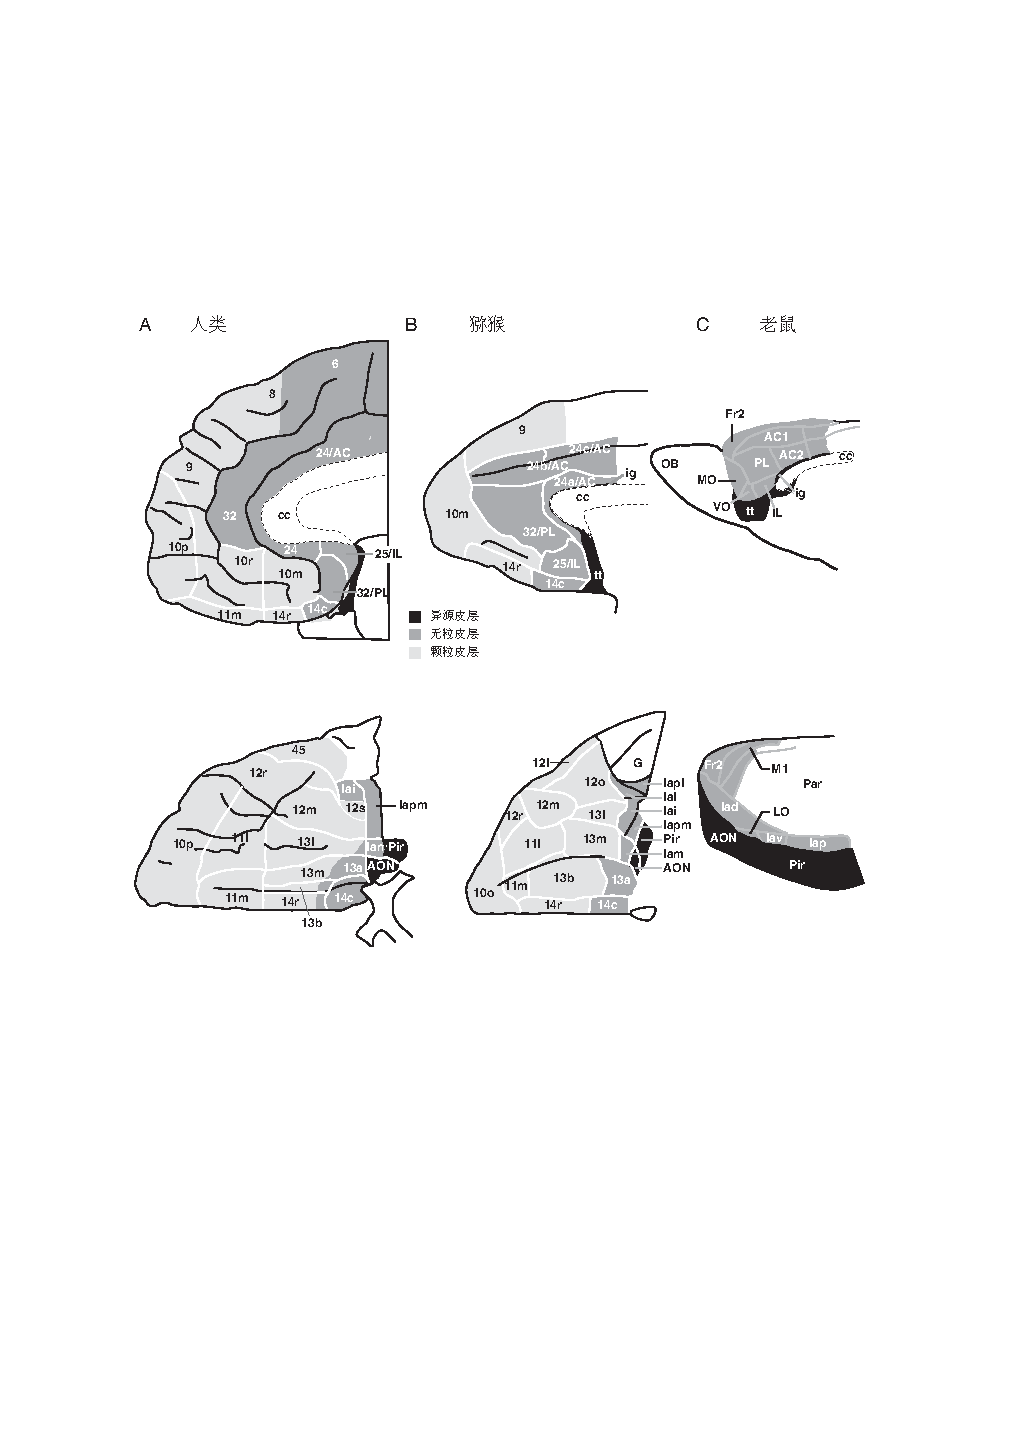
\includegraphics[width=0.8\linewidth]{image_pfc/Fig_2_1}
	\caption*{图2.1(A)人类前额皮层的内侧(上)和眶上区(下)(Ongur等人,2003)。 (B)猕猴前额皮层的内侧(上)和眶上区(下)(Carmichael&Price,1994)。 (C)老鼠前额皮层的内侧(上)和侧面(下)(Palomero-Gallagher&Zilles,2004)。在所有图中,向左为前端。上行:所有图中背面向上。下行:(A)和(B)中,侧面向上;在(C)中,背面向上。不按比例。缩写:AC,前扣带皮层;AON,前嗅“核”;cc,胼胝体;Fr2,第二额区;la,不含颗粒的岛叶皮层;ig,灰脑层;IL,下极叶皮层;LO,外侧眶上皮层;MO,内侧眶上皮层;OB,嗅球;Pir,锥体(嗅觉)皮层;PL,前扣带区;tt,盖带;VO,腹侧眶上皮层。区域细分标记为尾部(c);下(i);侧面(l),内侧(m);眶上(o),后部或极端(p),前端(r),或按任意标记(a,b)。 (A)改编自Ongur D. Ferry AT,Price JL。《人类眶上和内侧前额皮层的建筑分区》,《比较神经解剖学杂志》460:425-49,©2003,经John Wiley和Sons许可使用。 (B)改编自Carmichael ST,Price JL.《猕猴颅内和眶上前额皮层的建筑分区》,《比较神经解剖学杂志》346:366-402,©1994,经John Wiley和Sons许可使用。 (C)改编自Palomero-Gallagher N,Zilles K.《大鼠神经系统》中的异皮层.ed.G Paxinos,pp.729-57.圣迭戈,加利福尼亚州:爱尔斯维尔学术出版社。}
\end{figure}

非颗粒性前额叶皮层区域包括下肢内侧皮层、前扣带皮层、无颗粒的岛叶皮层、无颗粒的眶上皮层和前扣带回。在不同物种中,这些区域往往有不同的名称。例如,啮齿动物的下肢内侧皮层与灵长类动物的25区大致相对应,von Bonin和Bailey将其称为FL区(图1.1)。

众所周知,许多神经科学家认为老鼠拥有与灵长类动物相同的前额叶皮层。并且他们坚持认为,老鼠具有模拟灵长类动物前额叶皮层的微型复制品,或者可以将其所有属性混合在他们的小型无颗粒区域中(Kolb 2007;Seamans等人2008;Schoenbaum等人2009)。虽然我们对此持有不同的观点,但有一个命题应该得到普遍接受:在进化历史的某个时刻,我们的某些祖先缺乏颗粒性前额叶皮层。然而,现在我们不再缺失它。鉴于这个历史事实,询问颗粒性前额叶皮层带来了什么优势似乎是合理的。

尽管不是每个人都同意图2.1所描绘的同源性,但没有人严肃地质疑现代啮齿动物的大脑缺乏颗粒状前额叶皮层这一事实。对于其他哺乳动物,有一点存在争议:有人认为狗(Rajkowska&Kosmal 1988)和猫(Rose&Woolsey 1948)具有颗粒状前额叶皮层区域。但当我们亲自检查组织学材料中,狗和猫所谓的颗粒状区域时,它们看起来很像猴子和啮齿动物的无颗粒区域。

正如第1章所述,这种争议可能是由于观察者缺乏成体系的知识方法所致。当Mackey和Petrides(2010年)在猕猴和人脑中观察到这个问题时,他们发现一些传统上被归类为无颗粒额叶区域的区域实际上在第4层细胞体密度上,与最尾端的区域相比有略微的增加。也就是说,这些区域具有较弱的非颗粒质细胞结构,而不是完全的无颗粒结构。在食肉动物和其他非灵长类哺乳动物中发现颗粒状PF皮层的报告,反映了这种属性。神经解剖学家们都认为,细胞从额叶轨道和内侧表面向头部移动时,第4层的厚度会持续增加。因此,无颗粒皮质是否在第4层完全消失并不重要。我们可以将第4层密度低于给定阈值的区域视为足够无颗粒这一标准,用于我们之后的研究中(如图2.2所示)。

尽管大鼠缺乏细颗粒前额皮层,但一些神经科学家仍认为,大鼠前额皮质的中部与灵长类动物的中侧颗粒前额皮层(区域46)同源(Kolb 2007; Seamans等,2008),尽管后者的是一个颗粒区域(也称为背外侧或周主前额皮层)。同样,还有一些人认为,大鼠前额皮质的侧部与灵长类动物的整个眶前颞皮质同源,包括其颗粒部分(Kolb 2007; Schoenbaum等,2009)。该论点基于解剖学、生理学和神经化学的相似性以及基于声称在老鼠和猕猴中的损伤效应的相似性。

\begin{figure}[!htb]
	\centering
	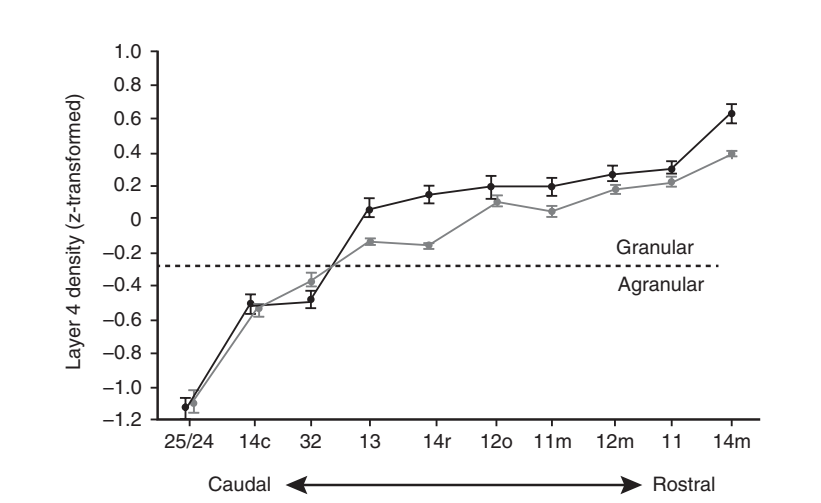
\includegraphics[width=0.8\linewidth]{image_pfc/Fig_2_2}
	\caption*{图2.2 显示了大脑额叶区域从尾向头发展的过程中,第4细胞层的归一化密度在猕猴(黑线)和人类(灰线)中的变化。误差条:SEM。该图由 Mackey S、Petrides M. 在《欧洲神经科学杂志》2010年32期(1940-1950页)中发表,经John Wiley and Sons出版社许可后再版。该图表明人类和猕猴大脑的腹内侧和侧壁眶前额皮质中具有可比较的成系统的区域。}
\end{figure}

然而,人们不能仅仅依据常被引用的相似性就推断其同源性。正如 Preuss(1995)所解释的那样,人们需要对特征进行诊断,即区分一组皮层区域和其他区域的特征。就像老鼠的非颗粒状前额皮质与猕猴的颗粒状前额皮质区域具有许多相似之处,例如编码估值的细胞。但是,这三个区域——老鼠的非颗粒状前额皮质以及猕猴的非颗粒状和颗粒状前额皮质——都具有与上述细胞同样的特性,其他皮层区域也是如此。因此,它们无法帮助我们理解前额皮层皮质的进化或建立其区域之间的同源性。例如,老鼠的非颗粒状区域的特性与灵长类动物的颗粒状前额皮质相似,但它们也与灵长类动物的非颗粒状前额皮质相似,那么这些特性就与动物的同源性无关。

有人声称,颗粒质前额皮层与丘脑中背核(MD)的联系是其诊断性特征(Rose和Woolsey,1948年;Akert,1964年;Uylings等人,2003年)。但是,MD核向实际上覆盖了额叶的几乎所有区域,包括颗粒质和非颗粒质区域。因此,与MD核的连接不能作为诊断性特征,故它们对于同源性的问题几乎没有影响或很少有影响。

曾经有一段时间,人们认为多巴胺能输入是颗粒状前额皮质的特征(Divac等,1978;Porrino&Goldman-Rakic,1982)。但是这些输入也终止于PF皮质的非颗粒状部分和运动前区,以及额叶以外大部分皮质。事实上,在灵长类动物中,多巴胺输入到运动前皮质和后枕叶皮质的强度比大多数颗粒状前额皮质都要强(Gaspar等,1992;Williams&Goldman-Rakic,1998)。因此,多巴胺输入不能帮助我们跨物种识别PF皮质。

最终,损伤结果得到了进一步的研究,例如对于延迟反应任务的研究结果。老鼠的前额内皮层损伤会导致该任务的障碍(Kolb等人,1974年),类似地,猕猴颗粒质前额皮层的损伤也会导致该任务的障碍(Goldman等人,1971年)。但是,前扣带回皮层的损伤也会导致猕猴在该任务上出现障碍(Meunier等人,1997年)。因此,该特征并非是诊断性的。我们将在第10章中更详细地讨论这个问题,老鼠和猕猴的障碍虽然表面上相似,但在重要的方面存在差异。

值得注意的是,我们并不是说灵长类动物拥有前额皮层而其他哺乳动物没有。我们认为非灵长类哺乳动物也有一些可以合理称之为前额皮层的区域。第3章和第4章将这些非颗粒质区域纳入了内侧和眶前颞皮层。但我们不赞同非灵长类哺乳动物具有类似于灵长类前额皮层的微型复制品或混合体的观点。非灵长类哺乳动物缺乏灵长类动物的颗粒质前额皮层以及执行其基本功能的任何区域。因为忽略了这些概念,文献中存在很多将非同源区域的结果混合在一起的实例,例如,引用灵长类动物的中侧前额皮层(46区)的研究结果来支持与啮齿动物的前额内皮层相关的某些结论。但其实这不是最好的方式。

我们对同源性的结论不应该引起太多争议。以视觉皮层为例,所有灵长类动物都共享10-20个视觉区域,其中有些物种甚至拥有更多的视觉区域(Kaas,2006年)。举个例子,一个被称为MT或V5的区域在视网膜中央凹有精细的专门分化功能,用于分析视觉运动。但老鼠的视觉区域少得多(Rosa和Krubitzer,1999年;Lyon,2007年),不可能复制灵长类动物10-20个视觉区域的所有功能,并且它们缺乏中央凹。另外,在缺乏中央凹的物种中进行视网膜中央凹的微观分析是不太可能的。

再以另一个例子为例,考虑到蝙蝠听觉皮层的回声定位功能。这些动物使用类似声纳的系统来检测它们与猎物的距离和猎物本身的速度。蝙蝠的听觉皮层有许多专门区域来处理与回声定位相关的声学信号,包括分析调频声音、多普勒频移等等(Suga等人,1997年;Fitzpatrick,1998年)。但如果老鼠的听觉皮层中的一些细胞也对类似的声音作出反应,这并不意味着它们执行与蝙蝠听觉细胞相同的功能。事实上,想象它们这样做是很奇怪的,因为老鼠不会用回声定位来追踪它们的食物。同样,认为老鼠的少数听觉区域具有与回声定位蝙蝠的大量专门区域相同的所有功能和属性是缺乏可信度的。

很少有神经科学家质疑这样一个想法:与老鼠共同祖先相比,声呐定位蝙蝠拥有新的听觉区域,而灵长类动物拥有新的视觉区域,以适应其在视觉敏锐度和色彩视觉方面的需求。同时,这些新区域支持新的功能,如对凹视动作或回声定位的分析,这一观点已经被广泛接受。因此,令人惊讶的是,同样的神经科学家们往往对这样一个想法犹豫不决:灵长类动物拥有新的前额区域,并且这些区域具有新的功能。

问题的一部分来自于使用“新”的词来描述区域或功能。有人提出,新的区域通过复制和随后的分化出现(Krubitzer&Huffman 2000)。如果是这样的话,那么合理的假设是,某些新区域的分化程度比其他区域低;当它们在许多哺乳动物中出现时,我们可以将更保守的区域识别为同源的。然而,在这样做时,我们需要认识到大多数进化所产生的变化都涉及到同源结构的修改,因此在物种之间具有绝对等价是不现实的。

相较于这些相对保守的区域,其他的复制产物则更加具有差异化,因此应该被称为新的区域。随着差异化的产生,它们开始执行新的功能,从而提供了优于其祖先状态的优势。然而,当这些新区域进化时,它们会与附近的区域共享属性,并且通常会与它们有轴突连接。因此,虽然PF皮层的颗粒层和无颗粒层部分具有许多共同特征。但是我们不应该基于此得出它们是同源或类似的结论。颗粒状的PF皮层专门在灵长类动物中进化而来,并发展为支持灵长类动物具有特别能力的区域。

\section{原猴亚目前额叶皮层}
灵长类动物 PF 皮层进化的最有力证据来自对丛林婴猴(眼镜猴属,也称为大婴猴属)的研究。鉴于这一证据的重要性,我们将详细地回顾它。然而,读者可以从本节末尾的摘要中了解该论点的要点。

讨论中必要地使用了一些可能不是所有神经科学家都熟悉的术语,因此表2.1列出了这些术语以便参考。主要的灵长类动物群组包括原猴亚目、原猴类、类人猿亚目和类人猿。在进化过程中,灵长类动物分裂成原猴类(湿鼻)(lemurs, lorises), 和丛林婴猴,构成了大多数称为原猴亚目的灵长类动物)和类人猿亚目(干鼻)(包括狐猴,人猿和类人猿)。类人猿亚目包括所有新大陆猴(Platyrrhines),以及旧大陆猴、大猩猩和人类(统称为狭鼻猿)。

\begin{table}[htbp]
	\centering
	\caption{本章中使用的生物学术语}
	\begin{tabular}{ll}
		\toprule
		术语 & 含义 \\
		\midrule
		进化 & 与祖先状态不同,具有差异化的  \\
		埃及古猿 & 一种已灭绝的类人猿,接近早期的狭鼻类动物  \\
		类人猿 & 猴子、猿类和人类  \\
		辛普森氏果猴 & 一个已经灭绝的古老哺乳动物类群  \\
		智利猴 & 一个灭绝的类人猿,接近于最早的阔鼻猴  \\
		狭鼻猿& 旧大陆灵长类动物(旧大陆猴、类人猿和人类),从阔鼻猿中分化出来  \\
		类人猿亚目& 眼镜猴与类人猿;从原猴类中分化出来  \\
		同源性& 从共同祖先继承而来的相似性,与由平行或趋同进化引起的相似性形成对比  \\
		旧大陆猴& 一组狭鼻猴类灵长目动物,包括猕猴、狒狒、长尾黑颚猴(绿猴)、白眉猴、长尾猴、山魈猴和红尾猴  \\
		副猿& 已灭绝的类人猿,接近于第一个类人猿,也被称为Simonsius  \\
		阔鼻猴& 新大陆猴,包括鬃狮猴、松鼠猴、枭猴和卷尾猴;从狭鼻猿中分化出来  \\
		更猴形类群& 已经灭绝的哺乳动物,可能是早期灵长类或早期灵长类的近亲,包括辛普森氏果猴  \\
		原始的& 类似于祖先的情况  \\
		原猴亚目& 原猴类灵长类动物和猴鼠目动物; 不构成一个天然类群  \\
		原猴类& 大多数原猴类灵长类动物,包括狐猴、懒猴和丛林婴猴;从类人猿中分化出来  \\
		\bottomrule
	\end{tabular}%
\end{table}%

接下来,我们假设现代灵长类动物和类人猿共有的特征可能存在于它们最后的共同祖先身上。由于那个祖先是早期的灵长类动物,因此我们认为这些特征也是早期灵长类动物的特征。我们还假设类人猿具有但灵长类动物没有的特征可能是在类人猿中进化出来的。像之前一样,在形成分支后,独立进化也在继续进行,因此灵长类动物可能具有类人猿所缺乏的适应性。

Preuss和Goldman-Rakic(1991a)认为,和几个其他颗粒状前额皮层区域一样,丛林婴猴的皮层缺乏中侧PF皮层(区域46)的同源区。相反,他们确定了尾部PF皮层(区域8)和眶上PF皮层的颗粒状部分的同源区。Preuss和Goldman-Rakic用各种论证支持了他们的结论,其中包括比较丛林婴猴和恒河猴的共同之处(Preuss&Goldman-Rakic 1991b)。他们还考虑了其他人在狐猴(另一种Strepsirrhine灵长类动物)上所做的工作。然而,他们大部分证据来自于对丛林婴猴和恒河猴前额皮层结构的研究。最近一项研究确认了他们所分析的大部分内容(Wong&Kaas 2010)。

\subsection{皮质结构}
图2.3显示了Preuss和Goldman-Rakic为丛林婴猴额叶皮层绘制的图。在本节中,我们将对其进行详细的介绍与分析,以供对解剖学细节感兴趣的读者参考。

首先,Preuss和Goldman-Rakic确定了运动前皮层的不含颗粒的区域(区域6)。在紧贴区域6的前额叶表面皮层上,包括一个独特的区域,具有“非常厚、密”的第4层和髓鞘化的纤维束,这些纤维束从皮质下白质向第4层延伸,在那里分散到更浅的层中。

Preuss和Goldman-Rakic得出结论,这个被称为后颗粒区(GrP)的区域(图2.3)与猕猴和人类的8区同源。在该区域的进行电刺激会引发灵长类动物(Wu等人,2000)和猕猴(Bruce等人,1985)的眼动作,这一发现支持了GrP区域包括前额眼场(FEF)的结论。

\begin{figure}[!htb]
	\centering
	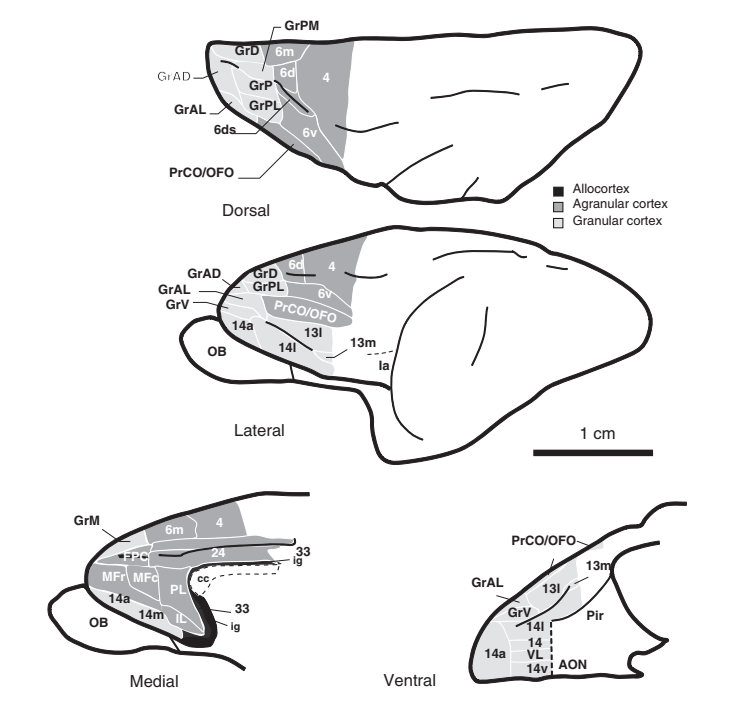
\includegraphics[width=0.8\linewidth]{image_pfc/Fig_2_3}
	\caption*{图2.3:灵长类动物丛林婴猴额叶皮层的建构图。所有图中,前端朝左。从上到下依次为背侧视图:向内为上;侧面视图:背侧向上;内侧面视图:背侧向上;腹侧面视图:侧面向上。缩略语如图2.1所示,包括以下内容:Gr,颗粒区,分为前部(A),背部(D),侧部(L),中部(M),后部(P);PrCO/OFO,前中央卷叶区/眶前额叶卷叶区;6ds,背区域6的沟部分;FPC,额极回扣带区;MF,中央前额叶皮质;VL,腹侧区域。摘自Preuss TM,Goldman-Rakic PS。灵长类动物狨和人猿类动物猕猴的颗粒前额叶皮层及其周围区域的髓样和细胞样结构。《比较神经学杂志》310:429-74 © 1991,John Wiley and Sons,获准使用。}
\end{figure}

Preuss和Goldman-Rakic指出,区域GrP在内侧被后-中颗粒区(GrPM)包围,在外侧被后-侧颗粒区(GrPL)包围(见图2.3)。他们认为GrPM和GrPL分别对应于8Ad区和45区的一部分。这个结论并不仅仅是基于它们与GrP和6区的拓扑关系。Preuss和Goldman-Rakic还指出,在灵长类动物和恒河猴的内侧和外侧区域中,锥形细胞比GrP区域小,横向定向的髓鞘束比GrP区域更显著。根据类似的基础,他们得出结论,更内侧的区域称为背颗粒皮层(GrD)和内侧颗粒皮层(GrM)(见图2.3),分别与恒河猴的8B区的背部和内侧部分同源。

Preuss和Goldman-Rakic稍微不那么自信地指出,他们推测了丛林婴猴的颗粒质PF皮层更向前部位的同源区,例如前背侧颗粒区(GrAD)。他们还考虑了两种可能性:一种是丛林婴猴的GrAD与猕猴和人类的区域8Ad的前部同源。这个想法基于GrP仅与猕猴的区域8Ad的尾部同源,留下其前部“自由区域”成为GrAD的同源区。另一种可能性是,GrP可能是猕猴的区域8Ad的前部和尾部的组合同源区。在这种解释下,区域GrAD可能与猕猴大脑中的后外侧PF皮层(区域9/46)同源,或者由于其与后顶叶皮层之间的联系不强,与极端PF皮层同源(Preuss 2007a)。这个问题还没有解决,但重要的是,Preuss和Goldman-Rakic没有发现GrAD与中侧PF皮层(区域46)对应的证据,这个结论受到了区域GrAD与后顶叶皮层之间连接较弱的支持。

至于眶额叶皮质,Preuss和Goldman-Rakic建议,丛林婴猴的腹侧颗粒区(GrV)可能对应于猕猴的11区(参见图1.2)。并且,总体而言,他们得出结论是丛林婴猴具有与猕猴差不多数量的眶部亚区。

Preuss和Goldman-Rakic无法确定类似于GrAL的区域在狨猴脑中的同源区,因此他们认为这个区域是在类狨目和类灵猴目分化后在狨猴中演化出来的。

作为他们最重要的观点之一,Preuss和Goldman-Rakic指出,许多猕猴大部分PF区域的髓鞘比额叶皮层的要少,而且在灵长类动物的额叶皮层中似乎不存在这样的髓鞘较少的区域。一项最近的结构成像研究将这个论点扩展到黑猩猩和人类中(Glasser等人,2011)。除了一些基于连接性的论证之外,他们得出了这样的结论:除非灵长类动物中的灰瘤质区域与其他动物有所不同,否则包括9、12/47和46区域以及可能的10区域在内的这些髓鞘较少区域在灵长类动物演化中是在单鼻亚目分化后进化出来的,而现代的猴子、大猩猩和人类通过继承拥有了它们。刚才提到的所有区域都具有灰质细胞形态学和少量的髓鞘,并且它们构成了现代人猿类,包括人类的大部分PF皮层。

\subsection{拓扑结构}
拓扑学术语指的是大脑皮层结构的空间排列方式,具体指皮层区域在二维皮层平面内的相对位置,可以想象将其展开以显示脑沟和脑回。例如,Preuss和Goldman-Rakic使用GrP与运动前皮质(区域6)之间的拓扑关系来确定它是短尾猴额叶眼区(FEF)的同源物。拓扑学术语在皮层进化的出版讨论中很少使用,但空间结构之间的证据一直是评估同源性最重要的特征之一。通常情况下,邻近结构为解释某些原本难以理解的结构提供了重要的指导,这是因为身体的基本模式在进化发育中是比较保守的特征之一。

前额皮层拓扑结构中一个特别重要的方面涉及它与异皮层的关系。如图2.1所示,一些前额区域直接相邻于黑色所示的异皮层。与大多数大脑皮层相比,异皮层仅有三个层次,其层次结构相对简单。典型的例子包括海马体和嗅叶皮层。

PF皮质的非颗粒部分靠近分配性皮层。例如,在啮齿类动物和灵长类动物中,无颗粒岛叶皮质毗邻嗅叶皮质和前嗅核。尽管前嗅核被称为“核”,但它是一种分配性皮质结构。其他非颗粒额叶区域,如前扣带皮质、下肢内侧皮质和前肢内侧皮质,毗邻更小、更不为人知的分配性皮层区域。虽然一些权威机构已经为靠近分配性皮层的皮层区域开发了复杂的名称,例如近分配皮层或前等皮层,但我们主要是基于比较的原因将它们全部视为新皮质的变体。

因此,非颗粒性前额皮质区域不仅可以通过其细胞结构进行识别,还可以通过它们与非皮层相邻来识别。相比之下,颗粒性前额皮质区域不与非皮层相邻,而是靠近非颗粒性前额皮质区域。因此,拓扑学和细胞结构都认为颗粒性前额皮质区域与非颗粒性前额皮质区域不同。需要注意的是,这种分析不包括运动皮层和前运动区,尽管它们也是非颗粒性的。

\subsection{皮质投射}
我们的论点也得到了某些皮质投射的支持。例如,在啮齿动物中,通常称为眶前额叶皮层或眶额皮层的区域向纹状体发送直接投射。仔细研究这个投射的细节提供了一些诊断特征,基于这样一个假设,即额叶皮层的同源部分向纹状体的同源部分投射。

在老鼠中,来自下肢内侧区和前扣带区的投射主要终止于伏隔核壳,这是腹侧纹状体的一部分(Brog等,1993; Reynolds&Zahm,2005)。纹状体分为两部分,腹侧纹状体包括伏隔核以及其他一些结构,而背侧纹状体包括尾状核和腹侧核。猕猴的25区和32区也投射到伏隔核壳(Haber等,1995,2006; Ferry等,2000),这一特征支持它们与啮齿动物中被称为下肢内侧区和前扣带区的区域的同源性。

在猕猴中,颗粒状前额皮层区域根本不投射到任何地方的伏隔核,更不用说它的壳了,它们也不投射到任何其他的腹侧纹状体区域。相反,它们投射到背侧纹状体的一部分,具体来说是尾状核(Selemon & Goldman-Rakic 1985)。因此,从详细的皮层-纹状体终止模式得出的结论与从细胞结构和拓扑学得出的结论一致。颗粒状前额皮层没有在老鼠中的同源物。

同样的规律也适用于眶前额叶皮层。在老鼠中,眶前额叶皮层投射到腹侧纹状体或其附近(Berendse等人,1992年)。在猕猴中,眶前额叶皮层的无颗粒部分(包括无颗粒岛叶区域)向这些纹状体部位发送大量的投射。但是,额叶皮层颗粒质部分投射到背侧纹状体。与半球外侧颗粒质PF区域一样,额叶表面的颗粒质区域主要投射到尾状核(Haber等人,1995年,2006年;Ferry等人,2000年;Öngür和Price,2000年)。

神经解剖学家描述了灵长类动物中新的前额叶皮层区域及其皮层纹理-尾纹突出部向腹侧移位的现象,将其称为“腹侧移位”(Schilman等人,2008年)。在老鼠中,非颗粒层的前额叶皮层投射于纹状体的背部和腹部之间。然而,在灵长类动物中,同源的非颗粒层的前额叶皮层的投射终止于纹状体的腹部三分之一位置。这种腹侧移位与新的前额叶皮层区域投射到更背部的纹状体区域是一致的。

我们在这里指出的现象,与那些认为啮齿动物的背内侧纹状体与灵长类动物的尾状核是同源的人存在分歧的主要原因是基于拓扑学(Balleine&O'Doherty 2010)。在啮齿动物中,内囊并没有像在灵长类动物中那样将尾状核与壳核分开。这使得在背纹状体内进行同源性分配变得困难,这也是为什么Balleine和O'Doherty得出他们的结论的原因。然而,他们的同源性观点几乎没有任何来自比较神经解剖学的支持。灵长类动物的尾状核的一个小的腹部可能在啮齿动物中有同源物。然而,尾状核的头部以及向其投射的纹状前额皮质区域是在灵长类动物中进化形成的。

此外,Preuss(1995)指出,在灵长类动物中,相比于灰质PF区的皮质-上丘(superior colliculus)弱的皮质-上丘投射,灰质PF区对皮质-上丘的投射更为强烈。然而,我们不认为这是一个主要的论点。虽然它适用于灰质PF皮层的背侧、内侧、腹侧、极性和尾侧,但眶上PF区对皮质-上丘的投射并不显著(Leichnetz等,1981)。